\documentclass[crop,tikz]{standalone}% 'crop' is the default for v1.0, before it was 'preview'
\usepackage{tikz,calc,pgfplots}
\usepackage{tikz-3dplot}
\usetikzlibrary{calc}
\usetikzlibrary{calc,patterns,decorations.pathmorphing,decorations.markings}
\usetikzlibrary{shapes.geometric}
\begin{document}

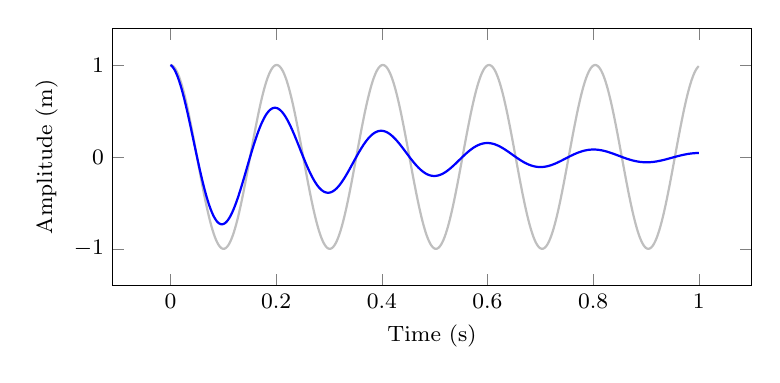
\begin{tikzpicture}[scale=1]
	\footnotesize
	\begin{axis}[
		width=0.8\textwidth,
		height=0.4\textwidth,
		xlabel={Time (s)},
		ylabel = {Amplitude (m)},
		xmax=1.1,
		ymax=1.4,
		ymin=-1.4,  
		samples=500]
		
		\def\wn{5*2*pi};
		\def\xo{1};
		\def\dxo{0};		
		\def\zEta{0.1};
		\def\wdd{sqrt(1-\zEta^2)*\wn};
		\def\Phii{rad(atan(\dxo/(\wdd*\xo)))};
		
		
		\addplot[gray!50!white, thick, domain=0:1] (x, {sqrt((\xo)^2+(\dxo/\wdd)^2) * cos(deg(\wdd*x- \Phii))});
%		\addplot[red,dashed, thick, domain=0:1] (x, {sqrt(\xo^2+(\dxo/\wdd)^2) * exp(-\zEta*\wn*x)});
%		\addplot[red,dashed, thick, domain=0:1] (x, {-sqrt(\xo^2+(\dxo/\wdd)^2) * exp(-\zEta*\wn*x)});	
		\addplot[blue, thick, domain=0:1] (x, {sqrt((\xo)^2+(\dxo/\wdd)^2) * cos(deg(\wdd*x- \Phii)) * exp(-\zEta*\wn*x)});
		
	\end{axis}
	
\end{tikzpicture}

\end{document}